\chapter{State of the Art}\label{chap:state-of-the-art}

Computer Algebra Systems (CAS) are mathematical software systems used in handling mathematical expressions involving abstract variables. Unlike a regular calculator, a CAS manipulates mathematical expressions symbolically, rather than numerically \parencite{bou2009computer}.

Such systems provide means to perform often tedious calculations not only in a faster way than a human could, but also in a more reliable way since they are not prone to human errors. They are used in a wide range of applications, from simple arithmetic to complex calculus, and are used in various fields such as engineering, physics, and mathematics.

However, the incentive to build these systems is not only to provide a tool for more efficient calculations, but also to circumvent the need for humans to perform what Lovelace called "the mechanical" section of the labors belonging to the mathematical sciences, and focus more on the parts of the work which require reasoning \parencite{lovelace1842sketch}.

\section{The Comprehensive System}\label{sec:the-comprehensive-system}

Davenport dates the first instances of computer algebra systems to 1953, when Kahrimanian and Nolan wrote their respective theses on analytical differentiation by means of digital computers \parencite{davenport1994computer}.

Nolan's work, a method which he dubbed the "Comprehensive System," enabled the programmer to write functions in an intermediate code that was then interpreted by a master program that allowed the Whirlwind I computer to perform the required operations using its standard subroutines \parencite{nolan1953analytical}. The main advantage of this system was it allowed the user to input the functions in a natural form, akin to how one would write them on paper.

As Nolan puts it, analytical expressions are "highly complex systems of coded information and can be written or orally stated in a number of different ways" \parencite{nolan1953analytical}. Thus, the challenge lies in finding a way to represent these expressions in a way that is both easy to input and easy to manipulate. His approach made use of a table of addresses each corresponding to a constant, a variable or an operation, taking advantage of Whirlwind I's instructions for special purposes, and the general procedure of the Comprehensive System was a sort of recusive divide-and-conquer algorithm, where the derivative to be computed was broken down into smaller, simpler derivatives to be computed.

The Comprehensive System and coetaneous pioneering works had to face one of the main challenges of computer algebra systems \parencite{davenport1994computer}, as strictly applying the rules of differentiation to a function can lead to an explosion of terms, many of which are redundant. This is known as the problem of expression swell \parencite{laue2019equivalence}, and it is a common problem in computer algebra systems. For the result to be useful, it is necessary to simplify the expression output by the system.

To illustrate this problem, consider the following example from Davenport's article \parencite{davenport1994computer}:

\begin{equation}
    \frac{\mathrm{d}}{\mathrm{d}x} \left( 2x + 3 \right) = 2 \times \frac{\mathrm{d}}{\mathrm{d}x} \left( x \right) + \frac{\mathrm{d}}{\mathrm{d}x} \left( 2 \right) \times x + \frac{\mathrm{d}}{\mathrm{d}x} \left( 3 \right)
\end{equation}

Although the result of this "literal" differentiation is correct, the expression is not simplified. One would expect the result to just be $2$. This shows that an extra layer needs to be applied to the system to rewrite the expressions given by the literal application of the operation rules, in order for it to be useful.

\section{The pioneering systems of the 1960s}\label{sec:the-pioneering-systems-of-the-1960s}

In the next decade, the 1960s, computer algebra programs were directly implemented in machine code, as a set of routines that were used by the programmer to perform the required operations \parencite{davenport1994computer}. In spite of this trend, some higher-level languages were starting to be used. The programming language Lisp, which makes use of symbolic expressions as its primary data structure \parencite{mccarthy1960recursive}, was created for computer algebra.

During this time, mathematicians Bryan John Birch and Peter Swinnerton-Dyer published their conjecture on elliptic curves. The Birch and Swinnerton-Dyer conjecture is an unsolved problem in number theory, and was developed with aid of the EDSAC-2 computer at the University of Cambridge \parencite{birch1965notes}, making use of the machine's computations to analyze a myriad of elliptic curves in the search of a trend among them. This was one of the earliest instances of computer algebra being used to aid in the development of a mathematical conjecture.

Davenport notes that three decades later the vast majority of computer algebra systems were still being written with a specific class of problems in mind, just like most of the programs from the 1960s \parencite{davenport1994computer}.

\subsection{Automatic integration: SAINT and SIN}\label{subsec:automatic-integration-saint-and-sin}

In 1961, as his doctoral disertation at MIT, James Slagle developed SAINT (Symbolic Automatic INTegrator), a heuristic-driven computer program that could solve symbolic integration problems, with a level of expertise similar to that of a "good college freshman" \parencite{slagle1963heuristic,geddes1992algorithms}.

The functions that SAINT could handle included real constants, variables, finite sums or finite products of elementary functions, elementary functions raised to elementary functions, trigonometric functions of elementary functions, and logarithmic or inverse functions of elementary functions \parencite{slagle1963heuristic}.

SAINT could perform transformations, trigonometric identities, substitutions, and other techniques to solve the integrals. It functioned on a system of goal-oriented rules, and Slagle estimated that it took an average of 2.4 minutes for it to finish solving an integration problem \parencite{slagle1963heuristic}.

Years later, Joel Moses presented SIN (Symbolic INtegrator) \parencite{moses1967symbolic}, also as part of his doctoral thesis. Unlike SAINT, the approach SIN took was more algorithm-driven, hence more efficient, solving the same set of problems in just 0.6 minutes on average, with many of the problems in the set being solved in just the first stage of SIN's subgoal algorithm. SIN also included a larger set of methods than SAINT. Interestingly, MATHLAB's rational function module was used for the development of SIN \parencite{moses1967symbolic}.

\subsection{MATHLAB, the first interactive system}\label{subsec:mathlab-68-the-first-interactive-system}

In 1968, during the yearly edition of the IFIP Congress, a computer algebra system called MATHLAB 68 (not to be confused with MathWorks's MATLAB, an unrelated programming language which first appeared around a decade later) was reported on through a paper \parencite{engelman1968mathlab} authored by Carl Engelman, one of the developers. Although the first MATHLAB system was presented in the year 1965 as the first interactive system designed to be used as a symbolic calculator, this version was an improved one, and it was also a successor to the Symbolic Mathematical Laboratory, another system developed by William Martin in 1967 \parencite{geddes1992algorithms}.

MATHLAB 68 was written in Lisp for the PDP-6 ITS system at the Massachussets Institute of Technology, and introduced many of the features that are now common in computer algebra systems, as will be explored in the following overview of the system. It was designed with modularity in mind, allowing extensibility of said modules, and even having different data representations suited for each of them. This, of course, meant that when communicating data between modules, a translation was necessary. According to Egelman, MATHLAB 68 shows "an overemphasis in its design compromises on programming ease," \parencite{engelman1971legacy} hinting at its small, disjointed team of developers as the likely cause of this. Despite this, many other, more modern, computer algebra systems are greatly in debt with MATHLAB 68.

The fact that MATHLAB systems were written in Lisp is not fortuitous, as Lisp was designed to be a language for symbolic computation \parencite{touretzky2013common}. In fact, many of their features were made possible by the use of Lisp. For example, MATHLAB 68's internal modules represent their data in one of two main ways: prefix expressions and rational expressions \parencite{engelman1971legacy}. The former are Lisp S-Expressions, that is, functional lists where the first element is the function and the rest are its arguments, such as \verb|(PLUS(TIMES A(EXPT 2)) (TIMES B X))| to represent the expression $ax^2 + bx$.

This representation, however, was not useful for manipulating polynomials, raising the need of the aforementioned rational expressions. These were recursive representations of polynomials, where a polynomial was represented as a list of the coefficients multiplying the powers of the variable, such as $x^2 + 4$ being represented by \verb|(1 0 4)|. The zero polynomial is represented as \verb|NIL| in this system. When a polynomial of $n$ variables was needed, it was represented as a list of the coefficients, which are also polynomials of $n - 1$ variables \parencite{engelman1971legacy}. This way, in order to represent the polynomial $ax^2 + a^2$, a second-degree polynomial in $x$, one would determine the coefficients are $a$ for the second-degree term, $0$ for the first degree term, and $a^2$ for the constant term. Because the non-zero coefficients are polynomials of $a$, they are in turn represented as \verb|(1 0)| and \verb|(1 0 1)|, respectively. Thus, the polynomial $ax^2 + a^2$ would be represented as \verb|((1 0) NIL (1 0 0))|.

The system handles the different representations of data from different modules by storing each of them. Representations of stored expressions were saved just as they were computed. This allowed users to look at past expression just as they would expect them, and in just a second of elapsed time \parencite{engelman1971legacy}.

MATHLAB 68 sported a sort of "lazy evaluation" utilizing Lisp's \verb|QUOTE| mechanism, which allowed the system to delay the evaluation of an expression or a function until it was needed. Contrary to the common practice, variables in MATHLAB 68 are quoted unless they are preceded by a single-quote mark (\verb|'|) \parencite{engelman1971legacy}. Engelman illustrates this difference by proposing that, if \verb|Y| is assigned the value of \verb|SIN(X)|, then \verb|DERIV(Y,X)| would evaluate to $\frac{\mathrm{d}y}{\mathrm{d}x}$ and, in contrast, \verb|DERIV('Y,X)| would evaluate to $\frac{\mathrm{d}}{\mathrm{d}x} \sin(x)$, "unquoting" (evaluating) the expression assigned to \verb|Y|. In order to actually find the derivative of $\sin(x)$, the command \verb|'DERIV('Y,X)| (evaluating both \verb|Y| and the result of the derivative) would return \verb|COS(X)|. If the user were to input \verb|'DERIV(Y,X)|, they may be surprised to find that the system would return \verb|0|, as \verb|Y| was not unquoted, therefore the system did not know that it was dependent on \verb|X|. If the user had declared this dependency beforehand, however, then the result would have been the same as with \verb|DERIV(Y,X)|.

This mechanism is symbolic of MATHLAB 68's design philosophy of preventing the system from making assumptions that rob the user of control over the data. The user is expected to prefer one of the two options, either quoting every variable by default or evaluating them. This design choice, as Engelman admits \parencite{engelman1971legacy}, is inferior to the approach of variables always being evaluated unless no value has been assigned to them.

User data was classified into one of three classes: expressions, equations and functions, each with their own behaviors when operated upon. Internally, these data types are differentiated by the leading term in their prefix representations. A prefix representation lead by the atom \verb|EQUAL| is identified as an equation, while one lead by the atom \verb|LAMBDA| is processed as a function. Any other representation not falling into one of these two categories is considered an expression \parencite{engelman1971legacy}.

The addition of two expressions is simply the result of concatenating them with a "\verb|+|" in between if the switch for simplification was turned off by the user. Adding an expression to an equation results in the expression being added to both the left-hand side and the right-hand side of the equation. Behavior for adding two functions is only allowed when the number of arguments is the same, and Engelman notes that the definition of function addition in MATHLAB 68 may not even be commutative when the functions being added contain free variables \parencite{engelman1971legacy}.

As for editing mathematical expressions, MATHLAB 68 had the top-level function \verb|TERM|, a substitute for a real editor that never came to be \parencite{engelman1971legacy}. This function works as an iterator, as \verb|'TERM(n,expr)|, where \verb|n| is (or evaluates to) a positive integer, returns the \verb|n|$^\text{th}$ term of the expression \verb|expr|. For example, if \verb|expr| is a sum, then the value would be the \verb|n|$^\text{th}$ summand, and if \verb|expr| is an equation, then the user could access the left-hand side by using \verb|'TERM(1,expr)| and the right-hand side by using \verb|'TERM(2,expr)|. The usage of this function is also allowed in an iterative fashion. This behavior is reminiscent to that of indexing and iterators in languages of the object-oriented programming paradigm, or to Lisp's own \verb|NTH| function, which returns a pointer to the specified component of the input list \parencite{touretzky2013common}.

User-defined functions in MATHLAB 68 were defined as macros, working as a substitution schema in most cases. When substitution is turned on, this can be quite powerful, as the user could define a function that is a substitution for a more complex expression, and then use this function in place of the expression. Additionally, with simplification turned on, all simplifications possible would be performed on the result of the function \parencite{engelman1971legacy}. Similarly, user-defined programs were defined as a collection of functions. Here is an example, taken from Engelman's paper, of a program that calculates the Runge-Kutta expansion for the solution of a differential equation $y' = f(x,y)$:

\begin{verbatim}
    PROG5(X1,X2,X3,X4,X5):X5$

    RUNGE1(X0,Y0):"('PROG5(
    (K1:'H*'F(X0,Y0)),
    (K2:'H*'F(X0+'H/3,Y0+'K1/3)),
    (K3:'H*'F(X0+2/3*'H,Y0-'K1/3+'K2)),
    (K4:'H*'F(X0+'H,Y0+'K1-'K2+'K3)),
    (Y0+E:I/8*('K1+3*'K2+3*'K3+'K4))
    ))$

    RUNGE2():"('PROG3 (
    (X0:'X0+'H),
    (Y0:'Y0+'K),
    'RUNGE1('X0,'Y0)
    ))$

    PROG3(X,Y,Z):Z$
    RUNGE():"(ANS('Y0,'RUNGE1(0,0),'RUNGE2(),'RUNGE2(),
    'RUNGE2(),'RUNGE2(),'RUNGE2(),'RUNGE2(),
    'RUNGE2(),'RUNGE2()$
    ))$
\end{verbatim}

Unquoting is disabled when inside double-quotation marks (\verb|"|), which allows the user to define functions that are not evaluated until they are called. MATHLAB 68 turns one of its quirks into a powerful feature, as it allows the user to define functions that are dependent on other functions, and then call them in a specific order.

The library of algorithms included in MATHLAB 68 contained a variety of functions, such as a greatest common divisor finder for polynomials, factorization of polynomials,  partial fraction expansion, direct and inverse Laplace transforms, integration of single-variable functions via Hermite's method \parencite{hardy1916integration}, among others.

Another one of these algorithms is \verb|SOLVE|, which tries to find the solutions to a rational equation for the variable specified by the user. The algorithm represents the result of the subtraction of the right-hand side to the left-hand side as a rational function and then tries to factorize the polynomial in the numerator. Roots are reported to the user as they are found, along with their respective multiplicities, but, because the algorithm will return a list of expressions, a form of data that is not considered in the system, the roots are not stored but instead given automatically generated names, which Engelman admits is a syntactical weakness of the system \parencite{engelman1971legacy}.

\verb|RATSIMP| (RATional SIMPlification) is another interesting one, as it ties into the way MATHLAB 68 handles expression simplification. This function is a simplifier for rational expressions, and it works by expanding all products, performing all greatest common divisor operations in order to cancel and factor the result and, finally, returning a single numerator and a single denominator \parencite{engelman1971legacy}. In doing so, \verb|RATSIMP| takes advantage of the recursive nature of the aforementioned representation of rational expressions. This algorithm is particularly powerful, and many of the other, more specific algorithms, depend on it, such as the partial fraction algorithm performing a sort of "reverse \verb|RATSIMP|".

However, the system already has a switch for simplification, called \verb|SIMP|. When this switch is turned on, the system will simplify the result of every operation, or so it should. MATHLAB's insistency in giving the user as many possibilities for representing a given expression becomes an obstacle for some of the simplification algorithms. For example, some complicated expressions may not be simplified automatically even when they are equal to zero, "a cardinal sin" in computer algebra systems \parencite{engelman1971legacy}. The general purpose simplification algorithm, based on work by Knut Korsvold \parencite{korsvold1966line}, eliminates the neutral elements of addition and multiplication, and performs all cancelations possible using an internal, temporary canonical representation of the expression. Engelman recounts that this same expression that the general purpose simplification algorithm was unable to simplify was then simplified by \verb|RATSIMP|, which was able to simplify the expression by expanding it and then canceling the terms.

As for matrix algebra, MATHLAB 68 also had routines written for it for handling matrices, such as a row-reduction algorithm for the inversion of matrices. The system is known to have been able to invert up to a $10 \times 10$ matrix \parencite{engelman1971legacy}.

Perhaps the most visually impressive, and another one of MATHLAB's firsts, was its output protocol, CHARYBDIS \parencite{millen1967charybdis}, a Lisp program written by Jonathan K. Millen. It was described as a two-dimensional output, where the system would print the expression in a way that would resemble how it would be written on paper. Since scientists at the time were not accustomed to Lisp's complicated parentheses-ridden output, having a way to display mathematical expressions in the universal two-dimensional form was a big advantage in getting mathematicians and other scientists to use computer algebra systems, and although plotters existed, they were slow and difficult to program, hence a solution for typewriter-like devices, which most computers already had for normal output, was the best compromise.

The program takes advantage of Lisp's lists, which are tree structures composed of atoms, and Lisp's recursion capabilities to traverse the tree and print the expression in a two-dimensional form. Here is Millen's demonstration of CHARYBDIS's output for the solution of the differential equation $Ay'' + By' + Cy = e^{x}$ \parencite{millen1967charybdis}:

\begin{verbatim}
                  - 1      2
        LOG(X) + -----LOG(X  + B*X + 1)
                   2
     + 
                 B                    2X + B
        - ----------------ARCTAN(----------------)
                   2                      2
           SQRT(- B  + 4)         SQRT(- B  + 4)
\end{verbatim}

With a simple grammar, a limited set of keywords, and an impressive dedicated output protocol, MATHLAB 68 was a system with never-before-seen features, hindered by some major weaknesses that its creators seeked to solve in the future \parencite{engelman1971legacy}.

\section{Libraries and language extensions}\label{sec:libraries-and-language-extensions}
Around the time MATHLAB 68 was presented, other computer algebra systems were being developed with a library-like approach, such as ALPAK and FORMAC, both based on the Fortran language \parencite{davenport1994computer}.

ALPAK was a library for Fortran intended for efficient manipulation of polynomials and rational functions. It featured four distinct data types: integers, rational numbers, polynomials and rational functions. It also featured truncated power series and matrices as data structures \parencite{brown1966language}.

FORMAC, on the other hand, was an extension of Fortran IV, and its main difference with the standard language it was based on was the representation of expressions: rather than as a series of computer instruction with a numerical value, they were a string of specially-coded symbols so, rather than Fortran's:

\begin{verbatim}
    X = 5.
    Z = 4.
    Y = X ** 2 + Z * 2.5/X.
\end{verbatim}

FORMAC would have:

\begin{verbatim}
    LET X = A + B.
        Z = 4.
    LET Y = X ** 2 + Z * 2.5/X.
\end{verbatim}

According to Davenport, these libraries and extensions were too difficult to use with proper storage management, and also algorithmically inadequate, hence their lack of success \parencite{davenport1994computer}.

\section{The Golden Age}\label{subsec:the-golden-age}

The 1970s are described as the Golden Age of computer algebra \parencite{davenport1994computer}. This is the time when the first general-purpose computer algebra systems were developed, such as Macsyma and Reduce. 

\subsection{Macsyma}\label{sec:macsyma}
After completing MATHLAB 68, Carl Engelman, William A. Martin and Joel Moses initiated a project to overhaul MATHLAB into a state-of-the-art computer algebra system \parencite{engelman1971legacy}. Although the project ditched most of the code from MATHLAB 68, it kept its heirarchical structure. The goal of Macsyma was to combine the results of Martin and Moses's respective research with Engelman's ideas from developing MATHLAB \parencite{martin1971macsyma}. It was written in Maclisp, a dialect of Lisp by the MIT's Project MAC, at which Macsyma was also being developed.

Macsyma was able to manipulate algebraic expressions automatically in a number of ways, such as limit calculation, symbolic integration, equation solving, simplification, and more.

Martin lists three main aspects of problem solving that should be taken into account by designers of interactive languages \parencite{martin1971macsyma}:

\begin{itemize}
    \item There are three types of errors in a command: lexical, syntactic, and semantic. The system should be able to detect, report and allow the user to correct these errors.
    \item The user must specify the level of evaluation desired, suited to the problem at hand.
    \item The system's language may be extended by the user either by renaming concepts already defined in the system, modifying concepts already defined in the system, or defining entirely new concepts.
\end{itemize}

There is a fourth aspect that Martin mentions as well, and that Macsyma is partiularly good at: the user and the system should interact in a form of discussion on the problem at hand. That is what MATHLAB was a pioneer in, as the first interactive computer algebra system. Macsyma's top-level editor allowed lines to be edited and retyped in case the user made a mistake \parencite{martin1971macsyma} (a feature Engelman expressed regret about not properly having in MATHLAB 68 \parencite{engelman1971legacy}), which was a big step forward in user interaction with computer algebra systems. Additionally, Macsyma automatically named each command and result, which allowed the user to refer to them later on.

Below is an example of a Macsyma session, taken from Martin's paper \parencite{martin1971macsyma}:

\begin{verbatim}
    (C1) D(MU,T):-3*MU*SIGMA$
    
    (C2) D(SIGMA,T):EPSILON-2*SIGMA**2$

    (C3) D(EPSILON,T):-SIGMA*(MU+2*EPSILON)$

    (C4) F[0]:1$

    (C5) G[0]:0$

    (C6) F[I]:=EXPAND(-MU*G[I-1]+DIFF(F[I-1],T))$

    (C7) G[I]:=EXPAND(F[I-1]+DIFF(G[I-1],T))$

    (C8) F[5]@
               2     3        2
    (D8) 105 MU SIGMA  - 15 MU  SIGMA

                             - 45 EPSILON MU SIGMA
\end{verbatim}

Martin's paper displays some examples of how Macsyma handles errors and allows the user to correct them, like using Macsyma's command \verb|SUBSTITUTE| to correct a typo in a command. In fact, the above session takes advantage of \verb|ALIAS| to abbreviate the name of the \verb|DERIVATIVE| command into just \verb|D|. This helps illustrate how Macsyma was truly designed with the user in mind, and how it fulfilled its objective of being a system that could interact with the user in a discussion-like manner.

Making the system even more customizable by the user, the \verb|TELLSIMP| facility allowed users to define their own simplification rules to add to the built-in simplification routine \parencite{martin1971macsyma}. This would push Macsyma to potentially be used in some areas and solve some problems it wasn't originally designed to.

Continuing with another one of MATHLAB's main features, Macsyma's different models and algorithms make use of special data types suited for each of them. What Moses \parencite{moses1971algebraic} called "radical" algebraic manipulation---where the user's expressions are transformed to a point where none of the original properties of the expression may be retained aside from its functional value---and its opposite, "conservative" algebraic manipulation, are met with Macsyma's general simplifier, which takes a stance in the middle of these two extremes, while the different modules of the system may delve more into one of these two extremes.

This hybrid approach allows for some manipulations typical of systems with a more radical approach on expressions that appear more conservative, like the ability to process $e^{2x} + 2e^{x} + 1$ as a quadratic polynomial in $e^{x}$ \parencite{martin1971macsyma}. This is a feature that was not present in most computer algebra systems of the time, and it is a testament to Macsyma's flexibility and power. It is achieved by Macsyma's use of two forms of representation for expressions.

The first one is called the "ordinary" form, and is reminiscent of Lisp and of MATHLAB 68's prefix expressions, using Reverse Polish Notation, like \verb|(times 3 (expt x 2))| for $3x^2$.

The second form is called the "canonical rational expression", or CRE, which is used internally and is much faster for manipulation of polynomials and rational functions \parencite{martin1971macsyma}. This form is very reminiscent of MATHLAB 68's approach to representing polynomials as trees. Polynomials are lists of at least three elements, with the first one being the variable, the second one being the degree of the polynomial and the third one onwards being the coefficients of the polynomial. So, $3x^2$ would be represented as \verb|(x 2 3)|, and $6x^2 + 4$ \verb|(x 2 6 0 4)|. Of course, just like MATHLAB allowed, coefficients may also be polynomials, allowing for expressions like \verb|(x 2 (y 1 1) 1 (z 1 7))| to represent $x^2y + 7xz$.

Many of the CRE commands in Macsyma are returning algorithms from MATHLAB, such as \verb|RATSIMP|, although Macsyma's versions are more efficient. However, some of the new commands in Macsyma, like \verb|RAT| or \verb|RATDISREP| are designed specifically to ease the conversions between forms of representation. Others, like \verb|FULLRATSIMP|, are expansions to the original commands. \verb|FULLRATSIMP| performs reductions on the expression until no more are possible \parencite{martin1971macsyma}.

Another interesting case is Macsyma's version of \verb|SOLVE|, which takes advantage of radical manipulations but doesn't return any strange-looking expressions resulting of these manipulations. Instead, it uses Macsyma's routines to expand expressions into polynomials and returns more general expressions \parencite{martin1971macsyma}.

Macsyma displays a more focused approach to algorithms than its predecessor, MATHLAB 68. It is apparant that its mission was to implement basic algorithms in the most efficient way possible \parencite{martin1971macsyma}, and it even went on to show that Lisp was a suitable programming language for computer algebra systems, a sort of flagship for the language in this field.

\section{The democratization of computer algebra}\label{sec:the-democratization-of-computer-algebra}

Up until the 1960s and 1970s, computer algebra systems were mostly experiments in research institutions \parencite{davenport1994computer}. Software was being developed with specific hardware in mind, hardware which was not available to the general public, as the computing requirements for computer algebra were too high \parencite{hearn2005reduce}.

Reduce, a general-purpose, physics-oriented computer algebra system developed by Anthony Hearn, put a focus on portability from the start of its development in 1963 \parencite{hearn2005reduce}. Originally, Hearn intended to write his system in Lisp to accomplish this goal, as the language was available in most machines of the time. However, the Lisp language was evolving into many different dialects, thus making the availability of "Lisp" in a machine not necessarily meaning that the system would run on it. Hearn's approach shifted to writing the system in a uniform subset of Lisp called Standard Lisp, which could be found in most machines either directly or by simple mappings to any other Lisp implementation \parencite{hearn2005reduce}.

In 1981, a portable Standard Lisp compiler was released, which allowed Reduce to be run on any machine that had a Lisp compiler and was compatible with the Standard Lisp protocols \parencite{hearn2005reduce}. This was a major step in luring new users to computer algebra systems. Reduce ended up becoming one of the most widely available systems of the decade \parencite{geddes1992algorithms}.

Many of the techiques used in a modern CAS can be traced back to the researchers at MIT. Macsyma's development kept going forward, keeping its focus on development and optimization of algorithms, making it the most powerful computer algebra system of the time \parencite{geddes1992algorithms}.

David Stoutemyer and Albert Rich, from the University of Hawaii, developed muMATH in the late 1970s, a general-purpose CAS and the first of its kind to be able to run on the IBM family of personal computers \parencite{geddes1992algorithms}. Being available on a small and accessible family of computers, muMATH opened the gates for a widespread use of computer algebra systems in research and in the classroom. It was implemented in the muSIMP programming language, an extension of the muLISP dialect of the Lisp language \parencite{derive-the-roots}.

Studies made in the 1980s and 1990s on the effects of employing computer algebra systems in the classroom, namely muMATH, showed that students who used the system had a better understanding of the material, although they evidenced that students unfamiliar with computers and software had trouble utilizing them \parencite{aspetsberger1984experiments,mayes1992effects}. The moment for computer algebra systems to be used in the classroom simply had not arrived yet, but the advantages were clear.

Despite these efforts, the majority of computer algebra systems had significant computer resource requirements, which prevented widespread use. Advances in computer hardware, however, would soon make these systems more accessible to the general public with the introduction of microprocessor-based workstations, and interest in portable computer algebra systems was reignited in the 1980s \parencite{geddes1992algorithms}.

Microprocessor-based workstations required even more efficiency in the algorithms and memory management of computer algebra systems, which made developers shift to languages like C, which let developers have more control over the memory and the execution of the system \parencite{geddes1992algorithms}.

This is the case of Maple, which was developed at the start by Keith Geddes and Gaston Gonnet at the University of Waterloo. Maple was written in C, with a modular structure, a light, easily-portable, compiled kernel, and a large library of routines (featuring integer and rational arithmetic and polynomial manipulation) written in the homonimous user-level programming language \parencite{geddes1992algorithms}. It was designed to provide user accessibility to computer algebra, inspired by the previous attempts at this of muMATH and in contrast to the large mainframe computers required to run Macsyma. The Maple system was also devised not to be tied to any operating system of programming language. \parencite{char1983design}.

Another focus that Maple had was on the user interface, which was created to be as user-friendly as possible, with a command-line interface that was easy to use and understand \parencite{char1983design}.

Maple featured a set of data structures used to represent programming language statements and types of expressions formed by arithmetic and logical operators, numbers, lists, sets, tables, symbolic functions, equations, ranges, procedures and series. All of these data structures were implemented in the Maple language as dynamic vectors at the machine level. They had a general format with each data structure being composed of a header encoding the length, type, simplification status and garbage collection status of the structure, and other fields containing data. This focus on dynamic vectors made the system very efficient in terms of memory usage and was integral to Maple's compactness \parencite{char1983design}.

Mathematica was another system developed in the 1980s, by Stephen Wolfram, and a major player in the field even today. It was also based on C, and it popularized integrated environments for computer algebra systems, with a notebook-like interface. It supported symbolics, numerics and impressive animated graphical capabilities, both two-dimensional and three-dimensional. Mathematica put on display how a CAS could benefit from the editing features on machines with graphical user-interfaces. \parencite{geddes1992algorithms}.

\begin{figure}[htb]
    \ffigbox[\FBwidth]
      {%
        \caption{Dini's surface, represented using Mathematica's graphical capabilities.}
        \label{fig:mathematica-dini}
      }%
      {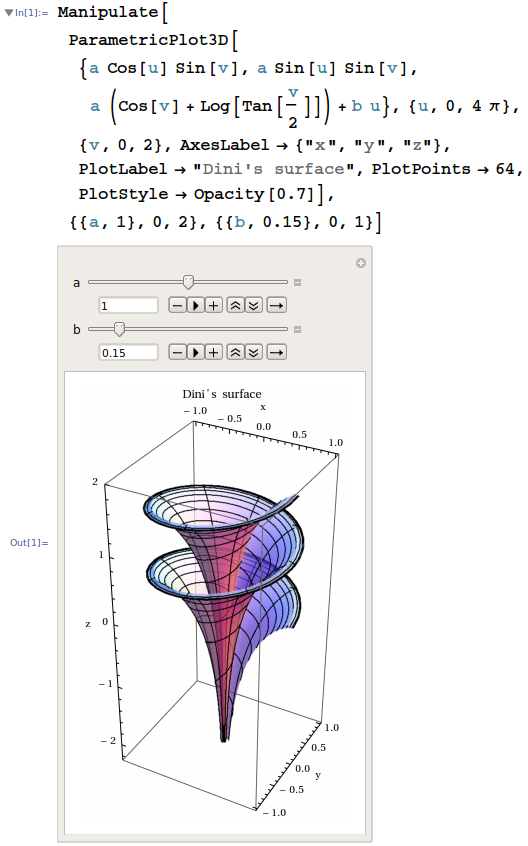
\includegraphics[scale=0.5]{mathematica-dini}}
\end{figure}  

Mathematica is divided into two parts: the kernel and the front end. The kernel is the core of the system, and it is responsible for the evaluation of expressions and the execution of commands. The front end is the graphical user interface, and it is responsible for the display of the results of the kernel's computations. The front end also allows the user to input commands and expressions, and it is responsible for the notebook interface, which allows the user to save the results of their computations in a document-like format. The front end also allows the user to edit the results of the computations, and it has a built-in help system that provides information on the system's commands and functions \parencite{wolfram1991mathematica}.

The Mathematica programming language can be used to write programs making use of the symbolic capabilities of the system, and it supports many programming paradigms, namely procedural programming, functional programming and rule-based programming \parencite{wolfram1991mathematica}.

Aside from new systems being developed, some of the systems designed in previous decades were still being developed and evolved. Macsyma, for example, was privatized by the Symbolics, Inc. \parencite{geddes1992algorithms} and kept being developed. DOE Macsyma, the name given to the MIT's version of Macsyma, was distributed by the United States Department of Energy, and eventually got rebranded to Maxima when it was released under the GNU Public License.

Derive, a successor to muMATH developed by Soft Warehouse, while not as powerful as other systems, provided a wide range of applications to 16-bit personal computers, a user-friendly interface two-dimensional input and editing of mathematical expressions, and both two-dimensional and three-dimensional graphics \parencite{geddes1992algorithms,derive-the-roots}.

The first pocket calculators featuring computer algebra capabilities were also released in the 1980s. Hewlett-Packard's HP-28C was the first \parencite{nelson-hp-calculator-first} pocket calculator to feature a computer algebra system. The HP-28 series of calculators featured algebraic manipulation, symbolic integration, Taylor series construction and symbolic solutions to algebraic equations \parencite{hp-28s-manual}. Texas Instruments followed suit in 1995 with the release of the TI-92, which featured a CAS based on Derive \parencite{ti-92-guidebook}.

\begin{figure}[htb]
    \ffigbox[\FBwidth]
      {%
        \caption{A screenshot of the TI-92's computer algebra system.}
        \label{fig:ti-92}
      }%
      {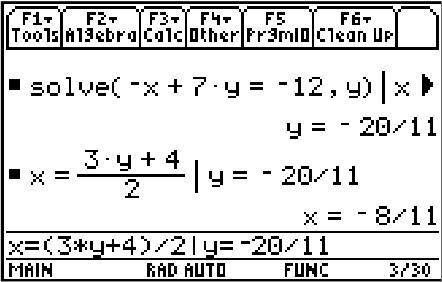
\includegraphics[scale=0.5]{ti-92}}
\end{figure}  

Democratization of computer algebra, of course, came hand in hand with their commercialization. Users would now have to pay for the software, which had both advantages and disadvantages. The biggest disadvantage was users not being informed enough to discern what "state of the art" computer algebra systems looked like, and were thus subjected to unrealistic claims on the matter. However, commercialization made the systems more user-friendly, more efficient, and widened their range of functionalities \parencite{geddes1992algorithms}.

\section{Current computer algebra systems}\label{sec:current-computer-algebra-systems}

Currently, computer algebra systems are more powerful and user-friendly than ever. They are used in a wide range of applications, from research to education, and they are available on a wide range of platforms, from personal computers to smartphones.

\subsection{Symbolic computation libraries}\label{subsec:symbolic-computation-libraries}

In his paper on the history of computer algebra \parencite{davenport1994computer}, Davenport already saw a trend towards computer algebra libraries. Today, this trend is more evident than ever, as many programming languages have libraries for symbolic computation.

\subsubsection{SymPy}\label{subsubsec:sympy}

One of the most popular symbolic computation libraries is SymPy, a Python library for symbolic mathematics. Debuting in 2005, and with over 500 contributors to the project, SymPy is open-source and free, and it is used by many people around the world for research, education, and industry. SymPy is written entirely in Python, and it is lightweight and easy to use. It features a wide range of mathematical functions, including algebraic manipulation, calculus, discrete mathematics, and more. SymPy is also extensible, and it can be used to build more complex mathematical software \parencite{meurer2017sympy}.

Among SymPy's many uses are calculus, category theory, combinatorics, geometry, matrices, polynomial manipulation, series, simplifications, solvers, statistics, and tensors. SymPy also has a code generation module that can be used to generate code in various languages, including C, Fortran, Julia and Python, among others \parencite{meurer2017sympy}.

SymPy's ease of use and availability at a general-purpose programming language like Python has made it key to many other projects, like the GNU Octave Symbolic Package or the Mathics and SageMath computer algebra systems \parencite{meurer2017sympy}.

\subsubsection{Symbolics.jl}\label{subsubsec:symbolics-jl}

Another, even more recent, popular symbolic computation library is Julia's Symbolics.jl. Julia is a high-level, high-performance programming language for technical and scientific computing. Symbolics.jl is designed to be fast, easy to use, and extensible, and it is used for a wide range of applications, including algebraic manipulation, calculus, differential equations, and more. Symbolics.jl is written entirely in Julia, and it is lightweight and easy to use. It features a wide range of mathematical features, such as symbolic arithmetic, symbolic polynomials, trigonometric functions, differentiation, symbolic linear algebra, automatic conversion of Julia code to symbolic code, function generation from symbolic expressions, support for non-standard algebras, and others. Symbolics.jl is also extensible, and it can be used to build more complex mathematical software \parencite{gowda2021high}. 

One of Symbolics.jl's greatest strengths is multiple dispatch, a notable feature of Julia. Multiple dispatch allows the definition of functions that adapt their behavior based on the types of their arguments, making Symbolics.jl highly flexible and powerful. This capability facilitates handling a wide range of mathematical problems effectively \parencite{gowda2021high}. The example that the official Julia documentation uses is quite illustrative: adding two integers is fundamentally different from adding two floating-point numbers, and both differ from adding an integer to a floating-point number. While these operations are implemented differently, they all represent the general concept of "addition". In Julia, these varied behaviors are encapsulated within a single object: the \verb|+| function \parencite{bezanson2017julia}.

\subsection{Communication among technologies}\label{subsec:communication-among-technologies}

Another one of the trends that Davenport foresaw in his paper was the communication among different technologies \parencite{davenport1994computer}. He argued that users of computer algebra systems would get used to one of the options available, even when other systems may be more efficient for a specific task. His idea was that a general-purpose system may need to call a system more specialized and more optimized in the area that the user is working on, or perhaps a specialized system would want to call a general-purpose system for tasks that were more efficiently implemented there, like polynomial manipulation.

SageMath is a computer algebra system that follows this idea. It is a free, open-source, general-purpose computer algebra system that is built on top of many other open-source mathematical software systems, including SymPy, Maxima, Singular, GAP, PARI/GP, FLINT, R, and many others.  It features a wide range of mathematical functions, including algebraic manipulation, calculus, discrete mathematics, and more. Interaction between all of these systems is made possible by a common Python-like language \parencite{stein2005sage,sagemath}.

\subsection{Computer vision}\label{subsec:computer-vision}

From the early days of computer algebra, a common challenge was designing a way for users to input mathematical expressions into the system in a way that was not too foreign to them. This is a challenge that has been tackled in many ways, and currently, with advances in computer vision, text recognition engines, and artificial intelligence, some computer algebra systems are able to recognize handwritten mathematical expressions and convert them into a format that the system can understand.

In 2014, Croatian startup MicroBlink released Photomath, a mobile application that uses computer vision to recognize handwritten mathematical problems and then solves them automatically \parencite{microblink-photomath}. The application uses the camera of a smartphone to capture the expression, processes the image to recognize the characters and symbols, and finally makes use a CAS to solve the problem and display the result. It is also a great tool for teaching students, as it provides clear, step-by-step instructions on how to solve the problem.

As of 2021, Photomath amassed over 220 million downloads \parencite{photomath-downloads}. Long gone are the days when computer algebra systems were a niche tool for researchers and mathematicians and muMATH's complexity confused students. Photomath is a testament to how far computer algebra systems have come, and how they are now accessible to anyone with a smartphone.

\begin{figure}[htb]
    \ffigbox[\FBwidth]
      {%
        \caption{Scanning a mathematical expression with Photomath.}
        \label{fig:photomath}
      }%
      {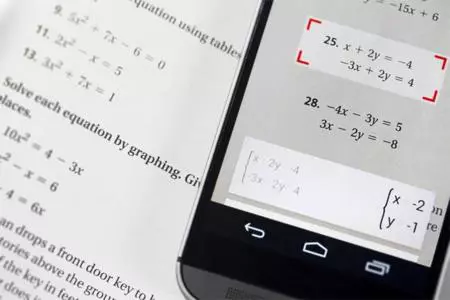
\includegraphics[scale=0.5]{photomath}}
\end{figure}

\begin{figure}[htb]
    \ffigbox[\FBwidth]
      {%
        \caption{Photomath interface showing the steps to solve a mathematical equation.}
        \label{fig:photomath-steps}
      }%
      {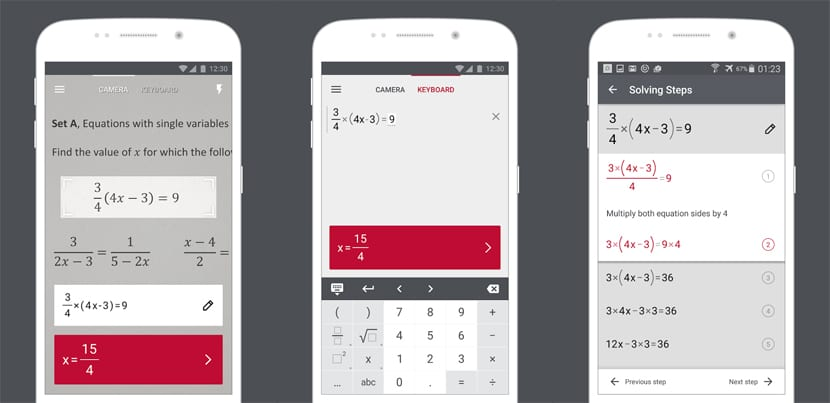
\includegraphics[scale=0.5]{photomath-steps}}
\end{figure}

\subsection{Answer engines and natural language processing}\label{subsec:answer-engines-and-natural-language-processing}

Possibly the most widely used tool for symbolic computation today is Wolfram Alpha. Released in 2009, Wolfram Alpha is a computational knowledge engine (or, more generally, an answer engine) that uses natural language processing to understand and answer questions posed by users \parencite{wolfram-alpha-about}.

Answer engines are not computer algebra systems, but they are systems that may employ a CAS in order to answer questions. Wolfram Alpha uses its older sister Mathematica to perform symbolic computations.

\begin{figure}[htb]
    \ffigbox[\FBwidth]
      {%
        \caption{Wolfram Alpha's interface showing its natural language input format and its symbolic computation and plotting capabilities, powered by Wolfram Mathematica.}
        \label{fig:wolfram-alpha}
      }%
      {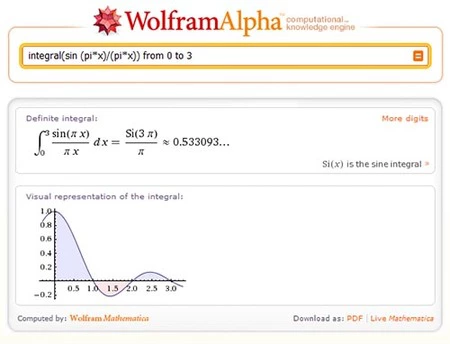
\includegraphics[scale=0.5]{wolfram-alpha}}
\end{figure}

Symbolab is another answer engine that uses a CAS to solve mathematical problems. It is a free, online tool that can solve a wide range of mathematical problems, including algebra, calculus, differential equations, and more. Symbolab has a similar interface to Wolfram Alpha, and uses a combination of natural language processing and symbolic computation to understand and solve problems posed by users step by step. Symbolab even features solutions for "word problems", making use of the advances of recent years in large language models to model elementary logical and mathematical problems \parencite{symbolab}.

\begin{figure}[htb]
    \ffigbox[\FBwidth]
      {%
        \caption{Symbolab's interface solving a word problem, displaying both its natural language processing and symbolic computation capabilities.}
        \label{fig:symbolab-word-problem}
      }%
      {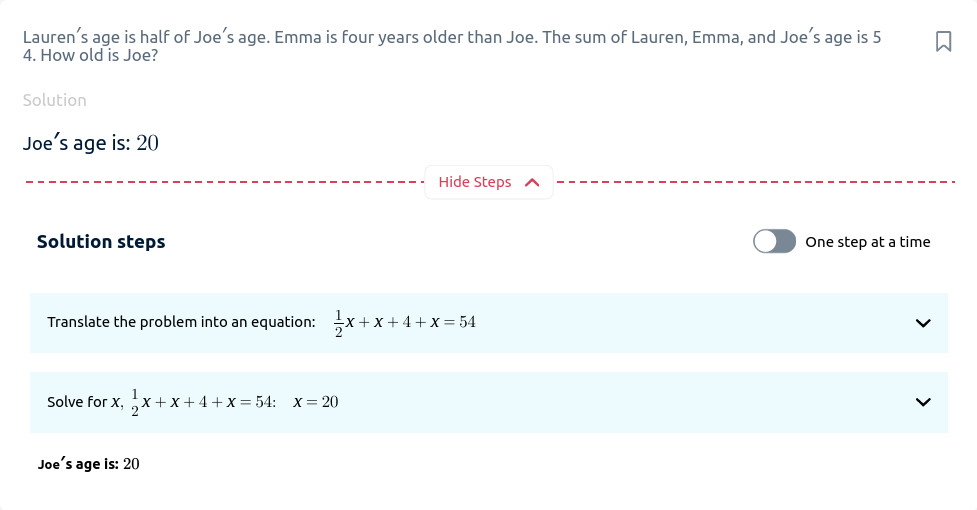
\includegraphics[scale=0.3]{symbolab-word-problem}}
\end{figure}

\section{Conclusion}\label{sec:conclusion}

Computer algebra systems have come a long way since their inception. From the early experiments in research institutions to the widespread use of answer engines and mobile applications, computer algebra systems have become an essential tool for researchers, educators, and students alike.

The democratization of computer algebra has been a key factor in the development of these systems. Advances in computer hardware, the development of portable computer algebra systems, and the availability of symbolic computation libraries have made computer algebra more accessible than ever. The integration of computer algebra systems with other technologies, such as computer vision and natural language processing, has further expanded their reach and made them more user-friendly.

The future of computer algebra systems is bright. With advances in artificial intelligence, machine learning, and natural language processing, we can expect to see even more powerful and user-friendly systems in the years to come. Future advances in the field may include more sophisticated natural language processing capabilities---perhaps even allowing users to ask questions about mathematical problems---, improved computer vision algorithms, and better integration with other technologies.

These systems will continue to play a key role in research, education, and industry, and will help us solve complex mathematical problems more efficiently than ever before.
